\section{\lego\ Design}
\label{sec:design}

Based on the \splitkernel\ architecture,
we built {\em \lego}, the first OS designed for hardware resource disaggregation.
\lego\ is a research prototype that demonstrates the feasibility of the \splitkernel\ design,
but it is not the only way to build a \splitkernel.
\lego' design targets three types of hardware components:
processor, memory, and storage,
and we call them {\em \pcomponent, \mcomponent}, and {\em \scomponent}.

This section first introduces the abstraction \lego\ exposes to users
and then describes the hardware architecture of components \lego\ runs on.
Next, we explain the design of \lego' process, memory, and storage \microos{}s.
Finally, we discuss \lego' global resource management and failure handling mechanisms.

Overall, \lego\ achieves the following design goals:

\begin{itemize}

\vspace{-0.1in}

\item Clean separation of process, memory, and storage functionalities.
\vspace{-0.1in}

\item Monitors run at hardware components and fit device constraints.
\vspace{-0.1in}

\item Comparable performance to monolithic Linux servers.
\vspace{-0.1in}

\item Efficient resource management and memory failure handling, both in space and in performance. % and performance-efficient memory replication scheme.
\vspace{-0.1in}

\item Easy-to-use, backward compatible user interface.
\vspace{-0.1in}

\item Supports common Linux system call interfaces.
\vspace{-0.1in}

\end{itemize}

\subsection{Abstraction and Usage Model}
\lego\ exposes a distributed set of {\em virtual nodes}, or {\em \vnode}, to users.
From users' point of view, a \vnode\ is like a virtual machine. 
Multiple users can run in a \vnode\ and each user can run multiple processes.
Each \vnode\ has a unique ID, a unique virtual IP address, %({\em \vip}),
and its own storage mount point. % ({\em \vmount}).
\lego\ protects and isolates the resources given to each \vnode\ from others.
Internally, one \vnode\ can run on multiple \pcomponent{}s, multiple \mcomponent{}s,
and multiple \scomponent{}s.
At the same time, each hardware component can host resources for more than one \vnode.
The internal execution status is transparent to \lego\ users;
they do not know which physical components their applications run on.

With \splitkernel's design principle of components not being coherent,
\lego\ does not support writable shared memory across processors. %execute application threads that need to have shared write access to common memory.
\lego\ assumes that threads within the same process access shared memory
and threads belonging to different processes do not share writable memory,
and \lego\ makes scheduling decision based on this assumption (\S\ref{sec:proc-scheduling}).
Applications that use shared writable memory across processes (\eg, with MAP\_SHARED)
will need to be adapted to use message passing across processes.
We made this decision because writable shared memory across processes is rare 
(we have not seen a single instance in the datacenter applications we studied),
and supporting it makes both hardware and software more complex 
(in fact, we have implemented this support but later decided not to include it because of its complexity).

One of the initial decisions we made when building \lego\ is to support the Linux system call interface 
and unmodified Linux ABI,
because doing so can greatly ease the adoption of \lego.
Distributed applications that run on Linux can seamlessly run on a \lego\ cluster
by running on a set of \vnode{}s. % and using their virtual IP addresses to communicate.

\subsection{Hardware Architecture}
\label{sec:hardware}
{
\begin{figure}[th]
\begin{minipage}{\figWidth}
\begin{center}
\centerline{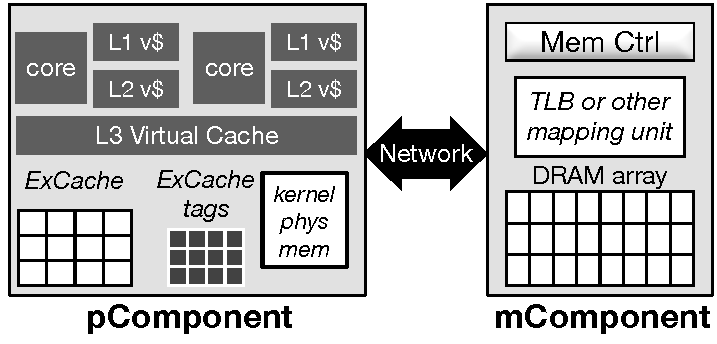
\includegraphics[width=2.8in]{Figures/hwarch.pdf}}
\vspace{-0.1in}
\mycaption{fig-hw-arch}{\lego\ \pcomponent\ and \mcomponent\ Architecture.}
{
}
\end{center}
\end{minipage}
\vspace{-0.15in}
\end{figure}
}

\lego\ \pcomponent, \mcomponent, and \scomponent\ are independent devices,
each having their own hardware controller and network interface (for \pcomponent, the hardware controller is the processor itself).
Our current hardware model uses CPU in \pcomponent, 
DRAM in \mcomponent, and SSD or HDD in \scomponent.
We leave exploring other hardware devices for future work.

To demonstrate the feasibility of hardware resource disaggregation,
we propose a \pcomponent{} and an \mcomponent\ architecture designed 
within today's network, processor, and memory performance and hardware constraints
(Figure~\ref{fig-hw-arch}).

\noindent{\textit{\uline{Separating process and memory functionalities.}}}
\lego\ moves all hardware memory functionalities to \mcomponent{}s 
(e.g., page tables, TLBs) and leaves {\em only} caches at the \pcomponent{} side. 
With a clean separation of process and memory hardware units, 
the allocation and management of memory can be completely transparent to \pcomponent{}s.
Each \mcomponent{} can choose its own memory allocation technique
and virtual to physical memory address mappings (\eg, segmentation). 

\noindent{\textit{\uline{Processor virtual caches.}}}
After moving all memory functionalities to \mcomponent{}s,  
\pcomponent{}s will only see virtual addresses and have to use virtual memory addresses to access its caches. 
Because of this, \lego\ organizes all levels of \pcomponent{} caches as {\em virtual caches}~\cite{Goodman-ASPLOS87,Wang-ISCA89},
\ie, virtually-indexed and virtually-tagged caches.

A virtual cache has two potential problems, commonly known as synonyms and homonyms~\cite{CacheMemory82}.
Synonyms happens when a physical address maps to multiple virtual addresses (and thus multiple virtual cache lines) 
as a result of memory sharing across processes,
and the update of one virtual cache line will not reflect to other lines that share the data.
Since \lego\ does not allow writable inter-process memory sharing,
it will not have the synonym problem.
The homonym problem happens when two address spaces use the same virtual address for their own different data.
Similar to previous solutions~\cite{OVC}, we solve homonyms by storing an address space ID (ASID) with each cache line,
and differentiate a virtual address in different address spaces using ASIDs.

\noindent{\textit{\uline{Separating memory for performance and for capacity.}}}
Previous studies~\cite{Gao16-OSDI,GU17-NSDI} and our own show that today's network speed 
cannot meet application performance requirements if all memory accesses are across the network. 
Fortunately, many modern datacenter applications exhibit strong memory access temporal locality.
For example, we found 90\% of memory accesses in PowerGraph~\cite{Gonzalez12-OSDI} go to just 0.06\% of total memory
and 95\% go to 3.1\% of memory
(22\% and 36\% for TensorFlow~\cite{TensorFlow} respectively,
5.1\% and 6.6\% for Phoenix~\cite{Ranger07-HPCA}).
%PG 90% 0.0063G 95% 0.301G 100% 9.68G
%TF 90% 0.608G 95% 0.968G 100% 2.7G

With good memory-access locality, we propose to %separate hardware memory into two categories and organize them differently:
leave a small amount of memory (\eg, 4\GB) at each \pcomponent{}
and move most memory across the network (\eg, few TBs per \mcomponent{}).
\pcomponent{}s' local memory can be regular DRAM 
or the on-die HBM~\cite{HBM-JEDEC,Knights-Landing},
and \mcomponent{}s use DRAM or NVM.

Different from previous proposals~\cite{Lim09-disaggregate}, 
we propose to organize \pcomponent{}s' DRAM/HBM as cache rather than main memory
for a clean separation of process and memory functionalities.
We place this cache under the current processor Last-Level Cache (LLC)
and call it an extended cache, or {\em \excache}.
\excache\ serves as another layer in the memory hierarchy between LLC and memory across the network.
With this design, \excache\ can serve hot memory accesses fast, while \mcomponent{}s can provide the capacity applications desire. 

\excache\ is a virtual, inclusive cache,
and we use a combination of hardware and software to manage \excache.
Each \excache\ line has a (virtual-address) tag and two access permission bits (one for read/write and one for valid).
These bits are set by software when a line is inserted to \excache\ and checked by hardware at access time.
For best hit performance, the hit path of \excache\ is handled purely by hardware
--- the hardware cache controller maps a virtual address to an \excache\ set, 
fetches and compares tags in the set, and on a hit, fetches the hit \excache\ line.
Handling misses of \excache\ is more complex than with traditional CPU caches, 
and thus we use \lego\ to handle the miss path of \excache\ (see \S\ref{sec:excachemgmt}).

Finally, we use a small amount of DRAM/HBM at \pcomponent{} for \lego' own kernel data usages,
accessed directly with physical memory addresses and managed by \lego. 
\lego\ ensures that all its own data fits in this space to avoid going to \mcomponent{}s.

With our design, \pcomponent{}s do not need any address mappings:
\lego\ accesses all \pcomponent{}-side DRAM/HBM using physical memory addresses
and does simple calculations to locate the \excache\ set for a memory access.
Another benefit of not handling address mapping at \pcomponent{}s and moving TLBs to \mcomponent{}s 
is that \pcomponent{}s do not need to access TLB or suffer from TLB misses,
potentially making \pcomponent{} cache accesses faster~\cite{Kaxiras-ISCA13}.
%We use software~\cite{softvm-HPCA97,Tsai-ISCA17} (\lego) to manage \excache\ and the kernel physical memory,
%although they can all be implemented in hardware too.

\subsection{Process Management}
The \lego\ {\em process \microos{}} runs in the kernel space of a \pcomponent\
and manages the \pcomponent's CPU cores and \excache. 
\pcomponent{}s run user programs in the user space.

\subsubsection{Process Management and Scheduling}
\label{sec:proc-scheduling}
At every \pcomponent, \lego\ uses a simple local thread scheduling model 
that targets datacenter applications 
(we will discuss global scheduling in \S~\ref{sec:grm}).
\lego\ dedicates a small amount of cores for kernel background threads 
(currently two to four)
and uses the rest of the cores for application threads.
When a new process starts, \lego\ uses a global policy to choose a \pcomponent{} for it (\S~\ref{sec:grm}).
Afterwards, \lego\ schedules new threads the process spawns on the same \pcomponent{} 
by choosing the cores that host fewest threads.
After assigning a thread to a core, 
we let it run to the end with no scheduling or kernel preemption under common scenarios.
For example, we do not use any network interrupts 
and let threads busy wait on the completion of outstanding network requests, 
since a network request in \lego\ is fast 
(\eg, fetching an \excache\ line from an \mcomponent\ takes around 6.5\mus).
\lego\ improves the overall processor utilization in a disaggregated cluster,
since it can freely schedule processes on any \pcomponent{}s without considering memory allocation.
Thus, we do not push for perfect core utilization when scheduling individual threads
and instead aim to minimize scheduling and context switch performance overheads.
Only when a \pcomponent{} has to schedule 
more threads than its cores will
\lego\ start preempting threads on a core.

\subsubsection{\excache\ Management}
\label{sec:excachemgmt}
\lego\ process \microos\ configures and manages \excache.
During the \pcomponent{}'s boot time, \lego\ configures the set associativity of \excache\
and its cache replacement policy.
While \excache\ hit is handled completely in hardware, 
\lego\ handles misses in software.
When an \excache\ miss happens, 
the process \microos\ fetches the corresponding line from an \mcomponent\ and inserts it to \excache.
If the \excache\ set is full, the process \microos\ first evicts a line in the set.
It throws away the evicted line if it is clean
and writes it back to an \mcomponent{} if it is dirty.
\lego\ currently supports two eviction policies: FIFO and LRU.
For each \excache\ set, \lego\ maintains a FIFO queue (or an approximate LRU list)
and chooses \excache\ lines to evict based on the corresponding policy (see \S\ref{sec:procimpl} for details).

\subsubsection{Supporting Linux Syscall Interface}
One of our early decisions is to support Linux ABIs for backward compatibility
and easy adoption of \lego.
A challenge in supporting the Linux system call interface is that 
many Linux syscalls are associated with {\em states},
information about different Linux subsystems that is stored with each process 
and can be accessed by user programs across syscalls.
For example, Linux records the states of a running process' open files, socket connections, and several other entities,
and it associates these states with file descriptors ({\em fd}s) that are exposed to users.
In contrast, \lego\ aims at the clean separation of OS functionalities.
With \lego' stateless design principle, each component only stores information about its own resource
and each request across components contains all the information that the destination component needs to handle the request.
To solve this discrepancy between the Linux syscall interface and \lego' design, 
we add a layer on top of \lego' core process \microos\ at each \pcomponent\ to store Linux states
and translate these states and the Linux syscall interface to \lego' internal interface.

\subsection{Memory Management}

We use \mcomponent{}s for three types of data:
anonymous memory (\ie, heaps, stacks), 
memory-mapped files, and storage buffer caches.
The \lego\ {\em memory \microos{}}
manages both the virtual and physical memory address spaces,
their allocation, deallocation, and memory address mappings.
It also performs the actual memory read and write.
No user processes run on \mcomponent{}s 
and they run completely in the kernel mode
(same is true for \scomponent{}s). 

\lego\ lets a process address space span multiple \mcomponent{}s
to achieve efficient memory space utilization and high parallelism.
Each application process uses one or more \mcomponent{}s to host its data
and a {\em home \mcomponent},
an \mcomponent\ that initially loads the process, 
accepts and oversees all system calls related to virtual memory space management
(\eg, \brk, \mmap, \munmap, and \mremap).
\lego\ uses a global memory resource manager ({\em \gmm}) to assign a home \mcomponent{} to each new process at its creation time.
A home \mcomponent\ can also host process data.

\subsubsection{Memory Space Management}
\noindent{\textit{\uline{Virtual memory space management.}}}
We propose a two-level approach to manage distributed virtual memory spaces,
where the home \mcomponent\ of a process makes coarse-grained, high-level virtual memory allocation decisions
and other \mcomponent{}s perform fine-grained virtual memory allocation.
This approach minimizes network communication during both normal memory accesses and virtual memory operations,
while ensuring good load balancing and memory utilization.
Figure~\ref{fig-dist-vma} demonstrates the data structures used. % in virtual memory space management.

At the higher level, we split each virtual memory address space into coarse-grained, fix-sized {\em virtual regions},
or {\em \vregion{}s} (\eg, of 1\GB).
Each \vregion\ that contains allocated virtual memory addresses (an active \vregion) is {\em owned} by an \mcomponent{}.
The owner of a \vregion\ handles all memory accesses and virtual memory requests within the \vregion.

{
\begin{figure}[th]
\begin{minipage}{\figWidth}
\begin{center}
\centerline{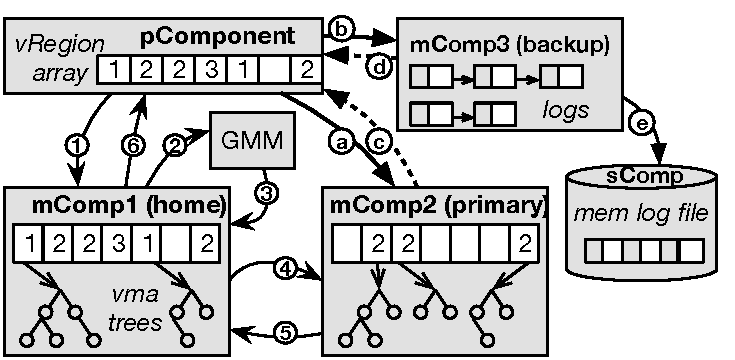
\includegraphics[width=2.8in]{Figures/dist-vma.pdf}}
%\vspace{-0.1in}
\mycaption{fig-dist-vma}{Distributed Memory Management.}
{
}
\end{center}
\end{minipage}
\vspace{-0.15in}
\end{figure}
}

The lower level stores user process virtual memory area ({\em vma}) information,
such as virtual address ranges and permissions, in {\em vma trees}.
The owner of an active \vregion\ stores a vma tree for the \vregion,
with each node in the tree being one vma.
A user-perceived virtual memory range can split across multiple \mcomponent{}s,
but only one \mcomponent{} owns a \vregion.

\vregion\ owners perform the actual virtual memory allocation and vma tree set up.
A home \mcomponent{} can also be the owner of \vregion{}s,
but the home \mcomponent{} does not maintain any information about memory that belongs to \vregion{}s owned by other \mcomponent{}s.
It only keeps the information of which \mcomponent{} owns a \vregion\ (in a {\em \vregion\ array})
and how much free virtual memory space is left in each \vregion.
These metadata can be easily reconstructed if a home \mcomponent{} fails.

When an application process wants to allocate a virtual memory space,
the \pcomponent{} forwards the allocation request 
to its home \mcomponent{} (\circled{1} in Figure~\ref{fig-dist-vma}).
The home \mcomponent{} uses its stored information of available virtual memory space in \vregion{}s
to find one or more \vregion{}s that best fit the requested amount of virtual memory space.
If no active \vregion\ can fit the allocation request, the home \mcomponent{} makes a new \vregion\ active and 
contacts the \gmm\ (\circled{2} and \circled{3}) to find a candidate \mcomponent{} to own the new \vregion.
\gmm\ makes this decision based on available physical memory space and access load on different \mcomponent{}s (\S~\ref{sec:grm}).
If the candidate \mcomponent\ is not the home \mcomponent{}, the home \mcomponent{} next forwards the request to that \mcomponent\ (\circled{4}),
which then performs local virtual memory area allocation and sets up the proper vma tree. 
Afterwards, the \pcomponent{} directly sends memory access requests to the owner of the \vregion\ where the memory access falls into
(\eg, \circled{a} and \circled{c} in Figure~\ref{fig-dist-vma}).


\lego' mechanism of distributed virtual memory management is efficient and it cleanly separates memory operations from \pcomponent{}s.
\pcomponent{}s hand over all memory-related system call requests to \mcomponent{}s
and only cache a copy of the \vregion\ array for fast memory accesses.
To fill a cache miss or to flush a dirty cache line, 
a \pcomponent{} looks up the cached \vregion\ array to find its owner \mcomponent{} and sends the request to it.

\noindent{\textit{\uline{Physical memory space management.}}}
Each \mcomponent\ manages the physical memory allocation for data that falls into the
\vregion\ that it owns.
Each \mcomponent{} can choose their own way of physical memory allocation
and own mechanism of virtual-to-physical memory address mapping.


\subsubsection{Optimization on Memory Accesses}
\label{sec:zerofill}
With our strawman memory management design, 
all \excache\ misses will go to \mcomponent{}s.
We soon found that a large performance overhead in running real applications 
is caused by filling empty \excache, \ie, {\em cold misses}.
To reduce the performance overhead of cold misses, we propose a technique 
to avoid accessing \mcomponent\ on first memory accesses.

The basic idea is simple: since the initial content of anonymous memory 
(non-file-backed memory) is zero, %undefined and can be any data, 
\lego\ can directly allocate a cache line with empty content
in \excache\ for the first access to 
anonymous memory instead of going to \mcomponent\
(we call such cache lines {\em p-local lines}).
When an application creates a new anonymous memory region, the process \microos\ records its address range and permission.
The application's first access to this region will be an \excache\ miss and it will trap to \lego.
\lego\ process \microos\ then allocates an \excache\ line, fills it with zeros, 
and sets its R/W bit according to the recorded memory region's permission.
Before this p-local line is evicted, it only lives in the \excache.
No \mcomponent{}s are aware of it or will allocate physical memory or a virtual-to-physical memory mapping for it.
When a p-local cache line becomes dirty and needs to be flushed, 
the process \microos\ sends it to its owner \mcomponent, which then
allocates physical memory space and establishes a virtual-to-physical memory mapping.
Essentially, \lego\ {\em delays physical memory allocation until write time}.
Notice that it is safe to only maintain p-local lines at a \pcomponent{} \excache\ 
without any other \pcomponent{}s knowing them, 
since \pcomponent{}s in \lego\ do not share any memory
and other \pcomponent{}s will not access this data.

\subsection{Storage Management}
\lego\ supports a hierarchical file interface that is backward compatible with POSIX 
through its \vnode\ abstraction. 
Users can store their directories and files under their \vnode{}s' mount points
and perform normal read, write, and other accesses to them.

\lego\ implements core storage functionalities at \scomponent{}s.
To cleanly separate storage functionalities, \lego\ uses a stateless storage server design, 
where each I/O request to the storage server contains all the information needed to 
fulfill this request, \eg, full path name, absolute file offset,
similar to the server design in NFS v2~\cite{Sandberg-NFS-85}.

While \lego\ supports a hierarchical file use interface,
internally, \lego\ storage \microos\ treats (full) directory and file paths just as unique names of a file
and place all files of a \vnode\ under one internal directory at the \scomponent{}.
To locate a file, \lego\ storage \microos\ maintains a simple hash table with the full paths of files (and directories) as keys.
From our observation, most datacenter applications only have a few hundred files or less.
Thus, a simple hash table for a whole \vnode\ is sufficient to achieve good lookup performance.
Using a non-hierarchical file system implementation largely reduces the complexity of \lego' file system,
making it possible for a storage \microos\ to fit in storage devices controllers that have limited processing power~\cite{Willow}.

\lego\ places the storage buffer cache at \mcomponent{}s
rather than at \scomponent{}s, because \scomponent{}s can only host a limited amount of internal memory.
\lego\ memory \microos\ manages the storage buffer cache by simply performing insertion, lookup, and deletion of buffer cache entries.
For simplicity and to avoid coherence traffic, we currently place the buffer cache of one file
under one \mcomponent{}.
When receiving a file read system call, the \lego\ process \microos\ first uses its extended Linux state layer to 
look up the full path name, then passes it with the requested offset and size to the \mcomponent\ that holds the file's buffer cache.
This \mcomponent\ will look up the buffer cache and returns the data to \pcomponent\ on a hit.
On a miss, \mcomponent\ will forward the request to the \scomponent\ that stores the file, 
which will fetch the data from storage device and return it to the \mcomponent.
The \mcomponent\ will then insert it into the buffer cache and returns it to the \pcomponent.
Write and fsync requests work in a similar fashion.

\subsection{Global Resource Management}
\label{sec:grm}
\lego\ uses a two-level resource management mechanism.
At the higher level, \lego\ uses three global resource managers for process, memory, and storage resources, 
{\em \gpm, \gmm}, and {\em \gsm}.
These global managers perform coarse-grained global resource allocation and load balancing,
and they can run on one normal Linux machine.
Global managers only maintain approximate resource usage and load information.
They update their information either when they make allocation decisions 
or by periodically asking \microos{}s in the cluster.
At the lower level, each \microos\ can employ its own policies and mechanisms to manage its local resources.

For example, process \microos{}s allocate new threads locally 
and only ask \gpm\ when they need to create a new process.
\gpm\ chooses the \pcomponent{} that has the least amount of threads based on its maintained approximate information.
Memory \microos{}s allocate virtual and physical memory space on their own.
Only home \mcomponent{} asks \gmm\ when it needs to allocate a new \vregion.
\gmm\ maintains approximate physical memory space usages and memory access load by periodically asking \mcomponent{}s
and chooses the memory with least load among all the ones that have at least \vregion\ size of free physical memory.

\lego\ decouples the allocation of different resources and 
can freely allocate each type of resource from a pool of components.
Doing so largely improves resource packing compared to a monolithic server cluster
that packs all type of resources a job requires within one physical machine.
Also note that \lego\ allocates hardware resources only {\em on demand}, 
\ie, when applications actually create threads or access physical memory.
This on-demand allocation strategy further improves \lego' resource packing efficiency
and allows more aggressive over-subscription in a cluster.

\subsection{Reliability and Failure Handling}
\label{sec:failure}
After disaggregation, \pcomponent{}s, \mcomponent{}s, and \scomponent{}s can all fail independently.
Our goal is to build a reliable disaggregated cluster that has the same or lower application failure rate
than a monolithic cluster.
As a first (and important) step towards achieving this goal, %building a reliable disaggregated cluster,
we focus on providing memory reliability by handling \mcomponent\ failure in the current version of \lego\ because of three observations.
First, when distributing an application's memory to multiple \mcomponent{}s, 
the probability of memory failure increases and not handling \mcomponent\ failure will cause applications to fail more often 
on a disaggregated cluster than on monolithic servers.
Second, since most modern datacenter applications
already provide reliability to their distributed storage data %(usually through some form of redundancy)
and the current version of \lego\ does not split a file across \scomponent,
we leave providing storage reliability to applications.
Finally, since \lego\ does not split a process across \pcomponent{}s,
the chance of a running application process being affected by the failure of a \pcomponent\ is similar to 
one affected by the failure of a processor in a monolithic server.
Thus, we currently do not deal with \pcomponent\ failure and leave it for future work.

A naive approach to handle memory failure is to perform a full replication of memory content over two or more \mcomponent{}s.
This method would require at least 2\x\ memory space,
making the monetary and energy cost of providing reliability prohibitively high (the same reason why RAMCloud~\cite{Ongaro11-RamCloud} does not replicate in memory).
Instead, we propose a space- and performance-efficient approach to provide in-memory data reliability in a best-effort way.
Further, since losing in-memory data will not affect user persistent data,
we propose to provide memory reliability in a best-effort manner.

We use one primary \mcomponent, one secondary \mcomponent, and a backup file in \scomponent\ for each vma.
A \mcomponent{} can serve as the primary for some vma and the secondary for others.
The primary stores all memory data and metadata. %, as discussed in \S~\ref{sec:}.
\lego\ maintains a small append-only log at the secondary \mcomponent{}
and also replicates the vma tree there.
When \pcomponent{} flushes a dirty \excache\ line, 
\lego\ sends the data to both primary and secondary in parallel (step \circled{a} and \circled{b} in Figure~\ref{fig-dist-vma})
and waits for both to reply (\circled{c} and \circled{d}).
In the background, the secondary \mcomponent\ flushes the backup log to a \scomponent{},
which writes it to an append-only file.

If the flushing of a backup log to \scomponent\ is slow and the log is full, 
we will skip replicating application memory.
If the primary fails during this time, \lego\ simply reports an error to application.
Otherwise when a primary \mcomponent\ fails, we can recover memory content 
by replaying the backup logs on \scomponent\ and in the secondary \mcomponent.
When a secondary \mcomponent\ fails, we do not reconstruct anything 
and start replicating to a new backup log on another \mcomponent{}.

